%% Use this line for the final version of your report
%\documentclass[final,american]{include/RaM/RaM-MScReport}

%% Use this line for the draft versions of your report, it enables rro/notes/line numbers/date in footer
\documentclass[lineno,UKenglish]{include/RaM/RaM-MScReport}

\settitle{Development of a myocardial perfusion phantom}
\setauthor{G.J. de Vries, s1854526}
%-------------------------------------------------------------------------------------------------
% This settings.tex contains settings required for *all* documents (reports, presentations, etc)
% Project or Report specific settings should go to their own settings files (eg CE/settings.tex)
% This file is included after the class definition and before project and report specific settings 
%-------------------------------------------------------------------------------------------------

%--------Useful packages (required by the example files, turn off if you do not use them)-------
\usepackage{babel}					% Add language specific support
%\usepackage{makeidx}				% Index support
%\usepackage[totoc,justific=RaggedRight]{idxlayout}	% Make last page of index balanced and add index to toc
\usepackage{caption}				% Provides means to style captions
%\usepackage{subcaption}				% Provides support for (sub)figures and (sub)tables
%\usepackage{float}					% Improved interface for floating objects (eg figures, tables, ...)
\usepackage{enumitem}				% Add styling support to (enumerate) environments
\usepackage{listings}				% Allows (external) source files to be shown in a syntax highlighted way
%\usepackage{amsmath}				% Provides miscellaneous enhancements for documents containing formulas
\usepackage{datetime}				% Provides commands for displaying the current time
%\usepackage{etoolbox}				% Provides \AtBeginEnvironment command
\usepackage{eurosym}				% Defines \euro command to display euro symbols
%\usepackage{appendix}				% Makes it possible to modify appendix numbering
%\usepackage{longtable}				% Allows tables to span multiple pages
%\usepackage{units}					% Shows units (eg m/s) in a nice way
%\usepackage{ctable}				% Provides \ctable command for the typesetting of table and figure floats
%\usepackage{ccaption}				% Support continuation captions (eg multi-page tables)
%\usepackage{verbatim}				% Adds verbatim environment, in which texts are exactly copied to the output
%\usepackage{pdfpages}				% Include PDF pages/documents in the current document
\usepackage{color, colortbl}
\definecolor{Gray}{gray}{0.9}

\usepackage{tabularx}

\usepackage{xfrac}

\usepackage{pdflscape}

\usepackage{multicol}

%%%%%%%%%%%%%%%%%%%%%%%%%%%%%%%%%%%%%%%%%
%%%%%%% Acronyms %%%%%%%%%%%%%%%%%%%%%%%%
\usepackage{acro}

%\DeclareInstance{acro-title}{empty}{sectioning}{name-format =}

\DeclareAcronym{CT}{
	short 	= CT,
	long 	= Computed Tomography,
	class 	= abbrev
}

\DeclareAcronym{MRI}{
	short	= MRI,
	long	= Magnetic Resonance Imaging,
	alt		= MR,
	class 	= abbrev
}

\DeclareAcronym{SPECT}{
	short	= SPECT,
	long	= Single-Photon Emission Computed Tomography,
	class	= abbrev
}

\DeclareAcronym{PET}{
	short 	= PET,
	long	= Positron Emission Tomography,
	class	= abbrev
}

\DeclareAcronym{MPI}{
	short	= MPI,
	long	= Myocardial Perfusion Imaging,
	class	= abbrev
}

\DeclareAcronym{PET-MR}{
	short	= PET-MR,
	long	= PET-Magnetic Resonance,
	class	= abbrev
}

\DeclareAcronym{AIF}{
	short	= AIF,
	long	= Arterial Input Function,
	class	= abbrev
}

\DeclareAcronym{CZT}{
	short	= CZT,
	long	= Cadmium Zinc Telluride,
	class	= abbrev
}

\DeclareAcronym{CAD}{
	short	= CAD,
	long	= Coronary Artery Disease,
	class	= abbrev
}

\DeclareAcronym{VC} {
	short	= VC,
	long	= Vena Cava,
	class	= abbrev
}

\DeclareAcronym{PA}{
	short				= PA,
	long				= Pulmonary Artery,
	long-plural-form 	= Pulmonary Arteries,
	short-plural		= s,
	class	= abbrev
}

\DeclareAcronym{PV}{
	short				= PV,
	long				= Pulmonary Vein,
	long-plural 		= s,
	short-plural		= s,
	class	= abbrev
}

\DeclareAcronym{PMT}{
	short			= PMT,
	short-plural	= s,
	long			= Photomultiplier Tube,
	long-plural		= s,
	class			= abbrev
}
%%%%%%%%%%%%%%%%%%%%%%%%%%%%%%%%%%%%%%%%%%%%%%%%
%%%%%%%%%%%%%%%% END ACRONYM %%%%%%%%%%%%%%%%%%%

\usepackage{include/files/requirements}

\iffinalversion
	\usepackage[final]{include/files/notes}% Add note commands, [final] removes all notes from the document
	\usepackage[final]{include/files/rro}  % Add Rich Report Outline support, [final] removes all RRO output from document
\else
	\usepackage{include/files/notes}       % Add note commands
	\usepackage{include/files/rro}         % Add Rich Report Outline support
\fi

% Add wrongly (or unknown) hyphened words here (space separated and - at possible hyphenation positions):
%\hyphenation{}

%% Spacing possibilities for captions are available as well
% See captions.pdf for all options!
\captionsetup{font=small,labelfont=bf}

%% Center all figures by default
%% http://tex.stackexchange.com/questions/2651/should-i-use-center-or-centering-for-figures-and-tables
\makeatletter
\g@addto@macro\@floatboxreset\centering
\makeatother

%% Make use small font size in verbatim environment
% Note: AtBeginEnvironment is provided by etoolbox package
%\AtBeginEnvironment{verbatim}{\small}

%% Include verbatim in the subfigure env
% From: subfig.pdf, section 4.4
% <Uncomment if verbatim is required in subfloat>:
%\makeatletter
%\newbox\sf@box
%\let\orig@subfloat\subfloat
%\renewenvironment{subfloat}[2][]%
%{ \def\sf@one{#1}%
%  \def\sf@two{#2}%
%  \setbox\sf@box\hbox
%  \bgroup}%
%{ \egroup
%  \ifx\@empty\sf@two\@empty\relax
%    \def\sf@two{\@empty}
%  \fi
%  \ifx\@empty\sf@one\@empty\relax
%    \orig@subfloat[\sf@two]{\box\sf@box}%
%  \else
%    \orig@subfloat[\sf@one][\sf@two]{\box\sf@box}%
%  \fi}
%\makeatother
%% Uncomment till here
  
%% Automatically provide H option for floats
% Requires float package
% \floatplacement{figure}{H} 
% \floatplacement{table}{H} 

%% abbreviation making
\newcommand{\abbr}[1]{(\textit{#1})}

%%lstlisting settings
\lstset{	%aboveskip=20pt,%
		numbers=none, %no line numbers
%		numbers=left, %show line numbers
		numberstyle=\tiny,%
		frame=single,%
		frameround={t}{t}{t}{t},%
		numbersep=5pt,%
%		language=C,% (default) code language in the document
		captionpos=b,%
		xleftmargin=2em,
		framexleftmargin=1.5em,
		xrightmargin=2em,
		framexrightmargin=1.5em,
		morecomment=[s][\itshape]{<}{>}, %also define <> as comment
		morecomment=[s][\itshape]{[}{]} %also define [] as comment
}

%lstinline with empty language definition
\lstdefinelanguage{empty}{}
\newcommand{\mylstinline}[1]{{\lstinline[language=empty]{#1}}}

% Default value of top separator (empty space) of lists
\setlist{topsep=4pt}

%% Don't show warnings like: ``PDF inclusion: found PDF version <1.x>, but at most version <1.4> allowed
% Uncomment if you experience these kind of warnings 
%\ifpdf
%	\pdfminorversion=6 
%\fi


\begin{document}
% Numbered roman style

\makerro				% Build RichReportOutline.rro file

\frontmatter


\includepdf{./frontpage/frontpage_r0d1.pdf}

% Use \maketitle or the available PDF when it is released (for student reports)
\maketitle

% Enter the name of the official RaM title page PDF between the brackets
% ! This method disables the option of using EPS files in your report.
% ! If EPS images are required, use LaTeX source instead of the PDF file
% 
\includepdf{./frontpage/frontpage_r0d1.pdf}
\cleardoublepage

% \include{Summary}
% Dutch summary is not obligatory
%\include{Samenvatting}

\chapter*{Preface}

\vskip-10pt
The system requirements specify all the requirements for the myocardial perfusion phantom. These requirements are based on research and interviews with stakeholders.

\vskip50pt
G.J. (Gijs) de Vries\\
Enschede, 7\textsuperscript{th} of January 2019
%In a two-sided printing style, it makes the next page a right-hand
% (odd-numbered) page, producing a blank page if necessary.
\cleardoublepage

% Add the table of contents pages (TOC)
\tableofcontents

% The report starts here
\mainmatter

% this contains a showcase of LaTeX
\chapter{Introduction}
\label{ch:Intro}

\rrod{Read into background information on D-SPECT}
\rrod{Write global background information}
\rrod{Introduce the rest of the document}
\rrod{Assignment was for dynamic SPECT scanning, but is that the same as using the D-SPECT? The D-SPECT can scan dynamically, and is available in ZGT}
\rrod{Too much SPECT detail in introduction? Moved to literature}
\rrot{Give arguments why to choose SPECT}

\Ac{MPI}, or, simply put, the imaging of the blood flow in the heart muscle, plays an important role in diagnosing heart failure or detecting \ac{CAD}. Imaging systems like \ac{CT}, \ac{MRI}, \ac{SPECT}, or \ac{PET} can visualise a (radioactive) contrast bolus in the supplying arteries and in underlying myocardial tissue, whose flow can give an indication of narrowed or blocked blood vessels.

Many variations in the visualisation process of myocardial perfusion, including variations in hard- and software, can (significantly) influence the outcome and in turn have consequences for patient treatment. These variations need to be validated against a well-known baseline.

The goal of the project is to develop a prototype myocardial perfusion phantom capable of repeated simulations of typical and cardiac defect situations using clinical software commonly used in myocardial perfusion scans. Most software packages require anatomical recognition points which imposes anatomical requirements on the phantom. In addition, the phantom can be used for educational and training purposes to demonstrate the impact of (poorly) chosen variables, e.g. pressure or flow, scanning parameters, cardiac defects, and so forth.

\section*{Document overview}
\label{sec:doc_overview}
\rrod{Update in correspondence with meeting december 10}
The project plan consists of a literature review of existing myocardial perfusion phantoms, their comparison to human physiology, and a discussion between the different types of scanners. The literature is followed by the research methodology containing the research questions and goals of the project. The detailed planning is the last section of the project plan stating workdays and -weeks, off-days, deadlines, and meetings.

\section*{Abbreviations}
\begin{multicols}{2}
	\printacronyms[include-classes=abbrev, name=Abbreviations, heading=none]
\end{multicols}

% add another chapter
% change file name for better descriptive names, but start with ch-
\chapter{Functional system overview}
This chapter goes into detail on the functional aspects of the myocardial perfusion phantom.
\section{Drivers}
\label{sec:drivers}
Many factors influence the outcome of \ac{MPI}. Some of these factors are:

\begin{tabular}{llll}
 	\multicolumn{1}{c}{\textbf{Tracer}} & \multicolumn{1}{c}{\textbf{Patient}} & \multicolumn{1}{c}{\textbf{Technology}} & \multicolumn{1}{c}{\textbf{Software}} \\
		- Concentration, & - Breathing artefacts, & - Modality, & - Package, \\
		- Volume, & - Cardiac motion, &  - Spatial resolution, & - Mathematical model, \\
		- Molecule size, & - BMI. & - Temporal resolution. & - Filters,\\
		- Injection speed.  & & & \makecell[l]{- \acs{ROI}.}\\
\end{tabular}

The strength of a phantom is that small modifications, for example, in contrast concentration or volume, or the mathematical model,  can be directly mapped to the outcome. It provides insight into dependent and independent factors in perfusion imaging.

Current phantoms either require modifications to software packages or do not model defects in a physiological way. Defects are typically modelled by reducing the flow through the myocardium by reducing the pump rate, effectively ignoring the complex relation between stenotic and non-stenotic arteries. Therefore, a myocardial perfusion phantom is needed that is compatible with clinical software and is able to mimic cardiac defects in a physiological way. This will increase the similarity with patient studies resulting in more reliable validation.

In addition to being a tool for validation of scanners and/or software packages, the phantom can be used for educational and training purposes to demonstrate the impact of hard- and software variables (sampling rate, \acf{ROI}, mathematical model), patient variables (BMI, blood flow and -pressure), tracer variables (concentration, type, injection speed), and many more.

\section{Approach}
The V-Model defines the project's development cycle. 

\subsection{Concept of operations}
\subsection*{Is the D-SPECT's dynamic scanning, in comparison with other modalities (CT, MRI, PET, or SPECT), suitable for quantitative myocardial perfusion imaging?}
\label{sec:concept_oper}
Quantitative flow measurements is made possible due to dynamic scanning. Dynamic scanning is not a newly emerged technique, it has been used with \ac{CT} in past research. Due to the solid-state detectors (Cadmium-Zinc Telluride), dynamic scanning is made possible for \ac{SPECT}. The D-SPECT is relatively new in the Netherlands. However, it has been employed in Japan, Canada, France, and Great-Britain. The D-SPECT is a highly specialised cardiac system. Due to the relatively small patient population, clinics often choose more all-purpose systems. The D-SPECT is very patient friendly due to its design in contrast to alternatives, e.g. GE uses a gantry design.

\ac{CT} is a well established modality with the highest spatial resolution. However, its largest drawback is that the radiation dose is directly proportional to the number of images, therefore increasing the likelihood of complication due to radiation exposure. \ac{MRI} does not rely an ionising radiation, but its lower temporal resolution makes it less suitable for dynamic imaging. \ac{SPECT} and \ac{PET} use radioactive tracers to image blood flow, thus exposing the patient to some degree of radiation. However, it is not directly proportional to the amount of images taken and is therefore less dangerous than \ac{CT}.

In addition, traditional \ac{SPECT} is, on average, 22\% less expensive than the current gold standard, \ac{PET}. D-SPECT is supposed to be even less expensive and faster. Furthermore, significant dose reduction, due to more sensitive solid-state detectors, reduces the strain and risk for patients. In addition, these solid-state detectors improve the image resolution. 

In summary, although the D-SPECT is relatively new in the Netherlands, it is more widely employed in Japan, Canada, France, and Great-Britain. The highly cardiac specialised system, its patient friendly design, the ability to scan faster and more accurate at significant dose reductions, make the D-SPECT suitable for quantitative myocardial perfusion imaging. 

\subsection{What must the myocardial perfusion phantom be able to simulate to validate quantitative MPI?}
At the most basic level, the phantom must be able to create an \ac{AIF}, either via the left ventricle or via an aorta, and simulate the perfusion in the myocardium. Furthermore, the phantom must be able to simulate the complex relation between stenotic and non-stenotic arteries in the myocardium; simply reducing the flow to the entire myocardium is not adequate. It should be possible, in case of simulated stenosis, to visualise the ischaemic tissue along non-ischaemic tissue.

Different kinds of compartment models exist for tracer kinetics. Initially, the phantom should simulate the compartment model consistent with clinical protocol. Additionally, other compartment models should be realisable by, for example, interchanging components.

\section{Business model}
The development of the myocardial perfusion phantom is primarily for the purpose of validating \ac{MPI}. An added benefit is the educational and training purpose. The phantom will distinguish itself from other phantoms due to its more true-to-nature design, ability to physiologically mimic cardiac defects, and the possibility of modelling different compartment models.

The primary focus remains on the current application of \ac{MPI} as performed at the ZGT in Hengelo, Overijssel.

\section{Requirements}
The functional requirements are summarised in table \ref{tab:funcreq}.

\begin{table}[h]
\caption{Functional requirements}
\label{tab:funcreq}
This table summarises the functional requirements for the prototype myocardial perfusion phantom.
\begin{tabular}{l|p{120mm}|}
	\makecell[l]{Requirement \\ number} & \multicolumn{1}{c}{Description}\\
	\hline
	FR01 & The phantom must be able to simulate blood flow, either using water of blood-mimicking fluid, at high flow rates (aortic flow). \\ 
	\rowcolor{Gray}
	FR02 & The phantom must be able to simulate blood flow, either using water or blood-mimicking fluid, at low flow rates (myocardial flow). \\
	FR03 & The high flow should be suitable for an \ac{AIF} extracted from the left atrium. \\
	\rowcolor{Gray}
	FR04 & Cardiac defects must simulate the complex relation between stenotic and non-stenotic arteries. \\
	FR05 & The phantom must be able to visualise (and measure) the 17-segment cardiac model. \\
	\rowcolor{Gray}
	FR06 & The phantom must use a 2-compartment model (simulating contrast uptake in tissue). \\
	FR07 & The contrast protocol must be equivalent to that used in clinical scans with D-SPECT. \\
	\rowcolor{Gray}
	\sout{FR08} & \sout{Contrast should be mixed equivalently to contrast mixing in patients.} \\
	\cline{2-2}
\end{tabular}
\end{table}

\section{Business and system use cases}	
The myocardial perfusion phantom is used by researchers with varying goals. Primarily, the phantom set-up is a tool to validate perfusion imaging hard- and software and to educate on independent and dependent factors, see section \ref{sec:drivers}. The researcher should be able to adjust the blood flow, both in the myocardium and in the aorta, and be able to set a cardiac defect.

Please note, setting the imaging and contrast parameters are not part of the phantom itself. 
\begin{figure}[!h]
	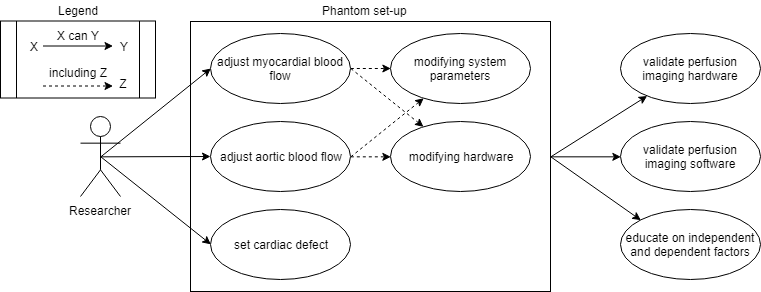
\includegraphics[width=\textwidth]{./images/usecase_diagram.png}
	\caption{Use case diagram for the prototype myocardial perfusion phantom}
	\label{fig:usecase}
\end{figure}

\section{Architectural overview}
A schematic overview of the flow set-up is shown in figure \ref{fig:funcarch}. The set-up consists of a flow generating system, e.g. mechanical pumps or pressure based, to generate the required aortic and myocardial flow, measuring systems, e.g. flow and pressure sensors, and the phantom itself, simulating the heart. The flow is controlled by means of a control system, over which the user has control. The flow parameters, i.e. flow and pressure, are measured by sensors which are monitored by a monitoring system. The monitoring system and control system cooperate such that user parameters are maintained. Figure \ref{fig:funcarch} shows a distinction between high and low flow, which is not a requirement. Low flow can be created by means of pressure difference in high and low flow circuit; increasing pressure in low flow circuit results in less volume passing through.
\begin{figure}
	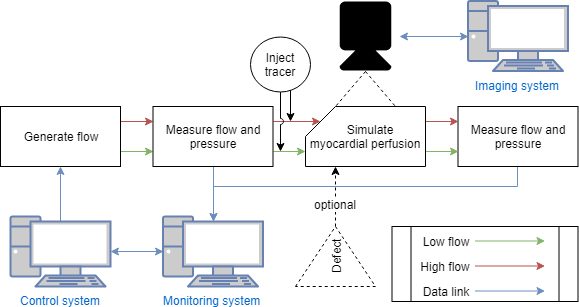
\includegraphics[width=0.75\textwidth]{./images/functional_architecture.png}
	\caption{Functional architecture for the myocardial perfusion set-up}
	\label{fig:funcarch}
\end{figure}

\chapter{Technical system overview}
\section{System}
The following section defines the phantom as described by \cite{van2011modeling}.
\subsection{Organ}
The organ to be simulated is the myocardium of the left ventricle, more specifically the blood flow in the myocardium. The left ventricle has a \ac{HLA} and \ac{VLA} cross-sectional shape of a horseshoe and a \ac{SA} cross-sectional shape of a circle, see figure \ref{fig:ventricle_shapes}. Quantitative data on blood flow is available in previous research by \cite{uren1994relation, chiribiri2013normal, ho2014dynamic, slart2015Pres}. Heart size indications are available in previous research by \cite{lin2008cardiac, maceira2006normalizedleft, maceira2006normalizedright}.

\begin{figure}[H]
	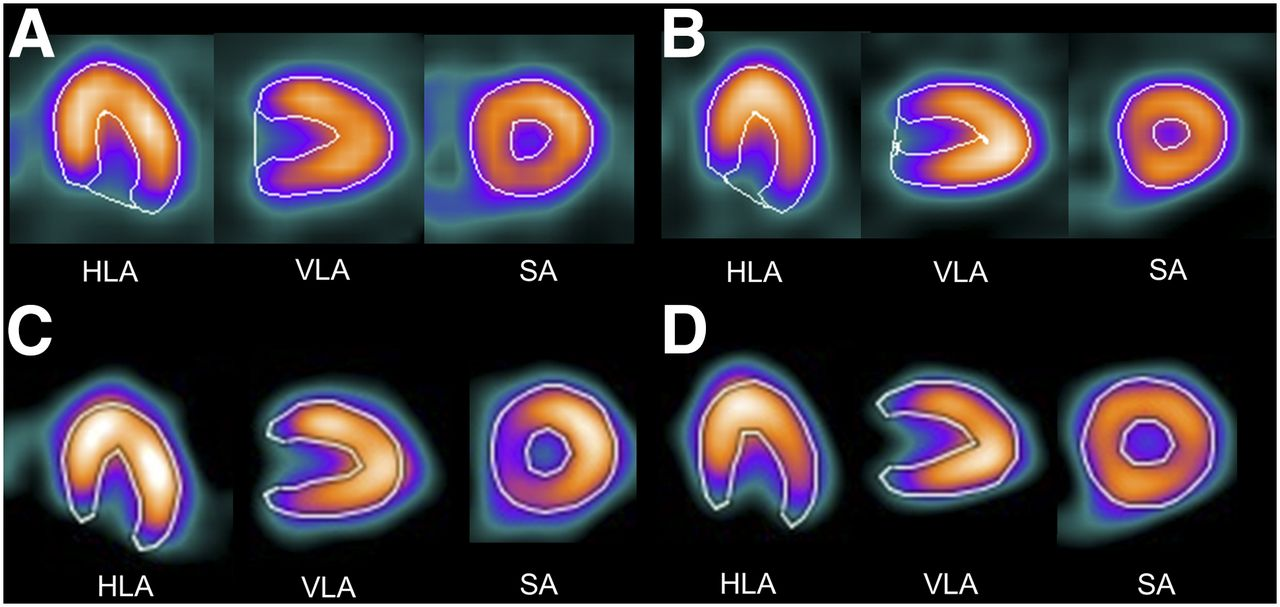
\includegraphics[scale=1]{./images/ventricle_shapes.jpg}
	\caption{Ventricle shapes in different planes\citep{yoneyama2017validation}}
	\label{fig:ventricle_shapes}
\end{figure}

\subsection{Population}
The heart phantom will be designed for average adults of both genders with ages between 18 and 79. The population consisted of patients with and without \ac{CAD}.
\subsection{Physiological states}
The heart will be simulated in both a resting state and in a stress state while the "patient" is in a supine position. The D-SPECT captures intensity images based on gamma rays caused by the radioactive decay of a tracer which is injected intravenously. The D-SPECT does not capture any information other than intensity information from gamma rays. Therefore the composition of the fluid is of less importance; water is most practical.
\subsection{Pathologies}
The phantom aims to simulate the perfusion in the myocardium of healthy patients and of patients with \ac{CAD}, more specifically stenosis of the coronary arteries or its subsequent branches. Stenosis in one of the arteries will have an impact on the overall flow behaviour (higher pressure, less overall flow, more flow to non-stenotic arteries) and thus requires the phantom to mimic the same behaviour.
\subsection{Clinical signs and monitored variables}
Blood flow is the most important variable to be monitored as these will be compared to the quantitative results produces by the processing software of the D-SPECT's images. Blood pressure must be monitored for indicative purposes. Depending on the phantom's final design, blood pressure can be critical for the simulation of the myocardial perfusion.
\subsection{Critical incidents}
No critical incidents will be simulated.
\subsection{Interventions}
No interventions will be simulated.
\subsection{Overall block diagram}
Figure \ref{fig:overall_block} shows an overview of all systems, how they are separated, and their interrelations. A distinction is made between four key elements; the flow set-up, the phantom, the imaging system, and external systems. The generation of an artificial heartbeat and the injection of the tracer are carried out externally and do not require development. Additionally, the imaging system (D-SPECT) with analysis software (4DM) do not require development since it concerns off-the-shelf hard-/software. The flow set-up and the phantom do require development. 

The flow is generated for different physiological states for high and low flows, i.e. for stress and rest. A closed-loop circuit monitors and controls the flow for optimal accuracy. The tracer is injected and flows to the phantom where the myocardial perfusion is mimicked. The contaminated water flows out of the phantom such that it can de disposed. Optionally, if the tracer can be filtered from the contaminated water, a closed, recirculating system can be fabricated; greatly reducing water waste. The tracer undergoes radioactive decay that results in the emission of gamma rays, which are picked up by the D-SPECT's detectors. The resulting intensity images can be reconstructed to form cross-sectional images which in turn are used to quantify the blood flow.

\begin{figure}[H]
	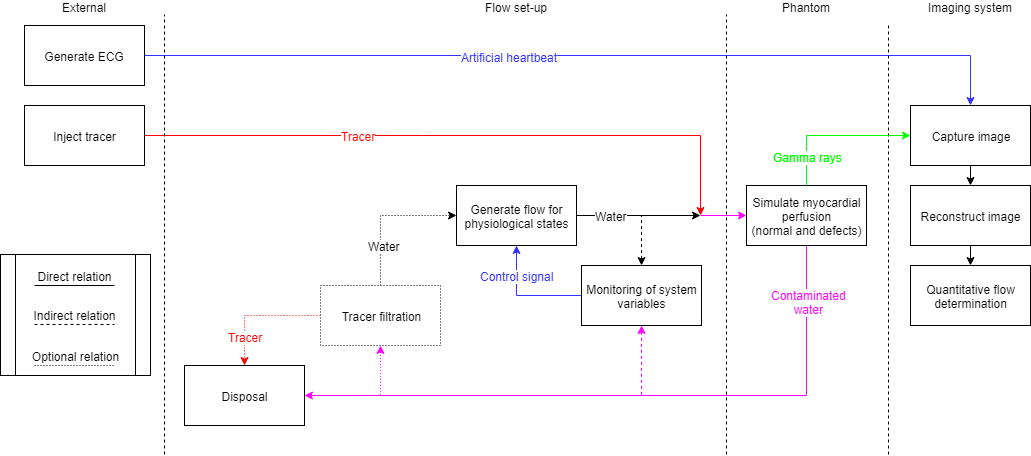
\includegraphics[width=\linewidth]{./images/technical_blockdiagram.png}
	\caption{Overall block diagram}
	\label{fig:overall_block}
\end{figure}

\section{Function requirements}
This section specifies the requirements set for the functions mentioned in figure \ref{fig:funcarch}.
\subsection{Generate flow}
In the project plan, a literature overview is given on perfusion phantoms, for a variety of organs, but also on physiological factors: perfusion rates, blood pressures, rates of stenosis et cetera. The TFR-GF requirements are based on the estimates by \cite{uren1994relation}, summarised in appendix \ref{app:physoverview}, \cite{chiribiri2013normal}, \cite{ho2014dynamic}, summarised in appendix \ref{app:physoverview_ho}, and \cite{slart2015Pres}.

Decisions and design choices are given in table \ref{tab:genflow_text}, quantitative requirements are given in table \ref{tab:genflow_quan}.

\begin{table}[H]
\caption{Textual requirements for function: Generate flow}
\label{tab:genflow_text}
\begin{tabular}{p{25mm}|p{115mm}|}
	\textbf{Requirement number} & \multicolumn{1}{c}{\textbf{Description}} \\
	\hline
	TFR-GFT01 & A variable, but constant, flow is to be generated, i.e. non-pulsatile. \\
	TFR-GFT02 & Flow generators need to be interchangeable. \\
	TFR-GFT03 & Flow feedback control for flow generators. \\
	\cline{2-2}
\end{tabular}
\end{table}

\textbf{TFR-GFT01} is based on reducing the complexity of the set-up. The ROI based AIF averages the intensity over time, which removes the pulsatile nature. Furthermore, the heart rate cannot be determine in the measurements results. Therefore, pulsatile flow is not a priority.
\textbf{TFR-GFT02} is based on maintaining flexibility such that the most optimal flow generator can be chosen based on the requirements for a specific experiment.

\textbf{TFR-GFT03} is based on ensuring reliability; no validation can be performed when the flow is not controlled.

\begin{table}[H]
\caption{Quantitative requirements for function: Generate flow}
\label{tab:genflow_quan}
\begin{tabular}{p{24mm}|p{65mm}ccp{21mm}|}
	\textbf{Requirement number} & \multicolumn{1}{c}{\textbf{Description}} & \multicolumn{1}{c}{ } & \multicolumn{1}{c}{\textbf{Value}} & \multicolumn{1}{c}{\textbf{Unit}} \\
	\hline
	TFR-GFQ01*	& Upper limit myocardial perfusion. 		 		& = 				& 300 				&  mL/min/100g \\
	TFR-GFQ02* 	& Lower limit myocardial perfusion. 				& = 				& 60 				& mL/min/100g \\
	TFR-GFQ03* 	& Typical perfusion rate during stress. 	 		& > \spacing < 		& 190 \spacing 300 	& mL/min/100g \\
	TFR-GFQ04*  	& Typical perfusion rate during rest. 			& > \spacing < 		& 60 \spacing 95 	& mL/min/100g \\
	TFR-GFQ05**	& Upper limit cardiac output.				 		& =					& 8 				& L/min \\
	TFR-GFQ06+		& Lower limit arterial pressure.				& =					& 56				& mmHg \\
	TFR-GFQ07+		& Upper limit arterial pressure.				& = 				& 155				& mmHg \\
	TFR-GFQ08		& Mean Arterial Pressure (MAP)\footnotemark. 	& = 				& 89				& mmHg \\
	TFR-GFQ09		& Typical MAP.								 	& > \spacing <		& \invchar 70 \spacing 110	& mmHg \\
	TFR-GFQ10 	& Feedback control accuracy 						& =					& 5					& \% \\
	\cline{2-5}
\end{tabular} \\
\raggedright
\textit{* combined flow to myocardium, indicated by blue arrows in figure \ref{fig:sim_heart}.} \\
\textit{** flow \textbf{not} entering the myocardium, indicated by red arrow in figure \ref{fig:sim_heart}.} \\
\textit{+ based on diastolic and systolic blood pressures, respectively. Measured at dashed line P in figure \ref{fig:sim_heart}.}
\end{table}

\footnotetext{Calculated as: $MAP \simeq DP + \sfrac{1}{3} (SP-DP)$}

\begin{figure}
\centering
\begin{minipage}{.5\textwidth}
  \centering
  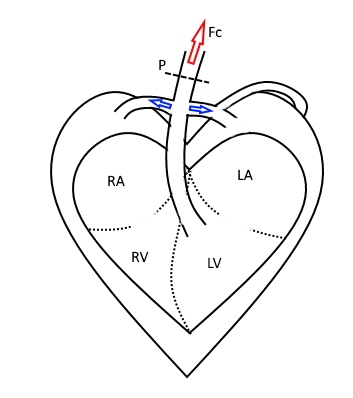
\includegraphics[width=0.7\linewidth]{./images/simplified_heart.png}
  \captionof{figure}{Simplified, schematic overview of the heart.}
  \label{fig:sim_heart}
\end{minipage}%
\begin{minipage}{.5\textwidth}
  \centering
  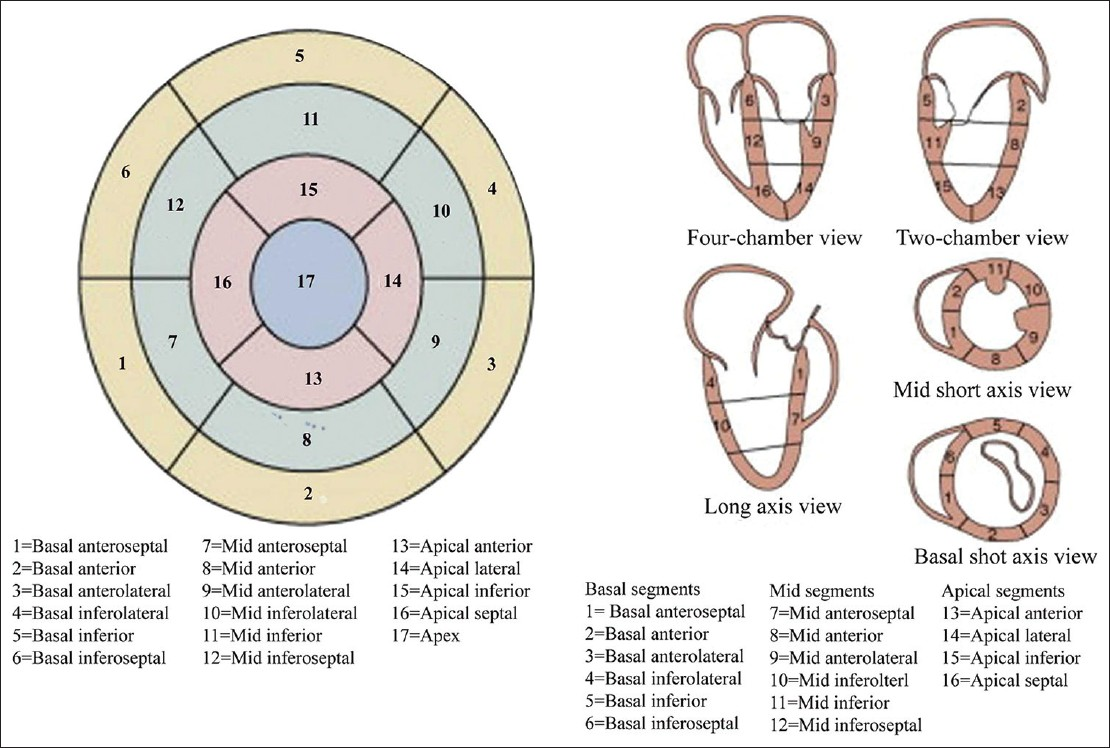
\includegraphics[width=0.95\linewidth]{./images/17_segment.jpg}
  \captionof{figure}{17-segment heart model}
  \label{fig:segment_heart}
\end{minipage}
\end{figure}

\subsection{Measuring flow and pressure}
This section focusses on the requirements for the measuring of the system variables; flow and pressure.
\begin{table}[H]
\caption{Quantitative requirements for function: Measure flow and pressure}
\label{tab:measflow_quan}
\begin{tabular}{p{25mm}|p{65mm}ccp{20mm}|}
	\textbf{Requirement number} & \multicolumn{1}{c}{\textbf{Description}} & \multicolumn{1}{c}{ } & \multicolumn{1}{c}{\textbf{Value}} & \multicolumn{1}{c}{\textbf{Unit}} \\
	\hline
	TFR-MFPQ01	& Flow measuring accuracy. 		 			 & <= 		& 5 		& \% \\
	TFR-MFPQ02 	& Pressure measuring accuracy.		 		 & <= 		& 5 		& \% \\
	TFR-MFPQ03 	& Absolute flow resolution.				 	 & >=	 	& 1 		& mL/min \\
	TFR-MFPQ04  & Sampling rate.					 		 & >= 		& 10 		& Hz \\
	\cline{2-5}
\end{tabular} \\
\raggedright
\end{table}

\begin{figure}[H]
	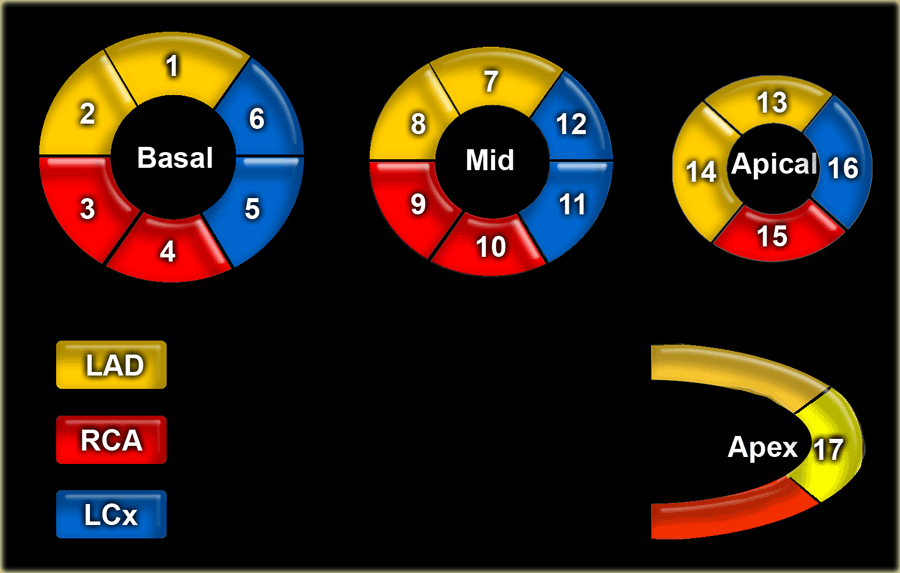
\includegraphics[width=0.5\linewidth]{./images/17_supply.png}
	\caption{Schematic representation of the supply to each segment (simplified).}
	\label{fig:segment_supply}
\end{figure}

\begin{figure}[H]
	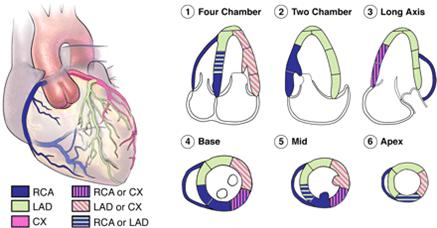
\includegraphics[width=0.5\linewidth]{./images/17_segment_2.jpg}
	\caption{Schematic representation of the supply to each segment.}
	\label{fig:segment_supply2}
\end{figure}

\subsection{Simulate myocardial perfusion}
This section specifies the requirements specified for the simulation of the myocardium.
\begin{table} [H]
\caption{Function requirements for function: Simulate myocardial perfusion}
\label{tab:funcsim}
\begin{tabular}{l|p{120mm}|}
	\makecell[l]{\textbf{Requirement} \\  \textbf{number}} & \multicolumn{1}{c}{\textbf{Description}}\\
	\hline
	\sout{TFR-SIMT01} & \sout{An \ac{AIF} must be extractable from the left ventricle, as per software requirement.}\\
	TFR-SIM02 & Stenotic arteries are mimicked in a physiological way by physically narrowing (or increasing flow resistance) of certain arteries. \\
	TFR-SIMT03 & Different stenotic severity, should be possible by, for example, variable flow resistors or interchanging components. \\
	TFR-SIMT04 & The phantom must be compatible with D-SPECT protocol. \\
	\hspace{1.5cm} A) & Flow to the myocardium is supplied by the RCA, LAD, and LCx. \\
	\hspace{1.5cm} B) & Flow for each segment is supplied individually by branches of the RCA, LAD, and LCx, see figure \ref{fig:segment_supply}. \\
	\hspace{1.5cm} C) & Flow from each segment is measured separately such that they can be compared to the 17-segment model. \\
	\hspace{1.5cm} D) & An ROI for the AIF can be taken in the left atrium. Alternatively, the ROI for the AIF can be taken in the left ventricle. \\
	\hspace{1.5cm} \sout{E)} & \sout{An AIF can be taken from the left atrium.} \\
	\hspace{1.5cm} F) & The left ventricle's myocardium has a Vertical and Horizontal Longitudinal Axial (VLA/HLA) cross-sectional shape of a horseshoe. \\
	\hspace{1.5cm} G) & The left ventricle's myocardium has a Short Axial (SA) cross-sectional shape of a circle. \\
	\hspace{1.5cm} H) & The phantom is oriented such that it mimics a patient in supine position. \\
	TFR-SIMT05* & Phantom's compartment model should match the currently practised protocol.\\
	\hspace{1.5cm} A) & The tracer specified in section \ref{sec:inj_tracer}.\\
	\hspace{1.5cm} B) & The contrast agent is absorbed by the myocardium to approximately 1.2\% of administered activity in 5 minutes. \\
	\hspace{1.5cm} C) & Contrast accumulates in skeletal muscles, spleen, liver, and kidneys (potential interference). \\
	\cline{2-2}
\end{tabular}
\raggedright
\textit{* \url{https://pubchem.ncbi.nlm.nih.gov/compound/131704316\#section=Absorption-Distribution-and-Excretion}}
\end{table}

\textbf{TFR-SIMT02} is based on the assumption that the relation between arteries, especially when some are narrowed, is too complex to be modelled independently. Simply reducing the overall flow in the myocardium will not capture that relation. Each segment of the left ventricle is supplied by a different branch of the three coronary arteries. One narrowed branch will have an impact on \textit{all} other branches, which leads to \textbf{TFR-SIMT03}. The severity of the stenosis will impact the other branches differently.

\textbf{TFR-SIMT04} is based on the goal of the project; to validate the D-SPECT. As mentioned in section \ref{sec:concept_oper}, the relatively less expensive, less invasive (patient friendliness and dose reduction), faster and more accurate system makes it suitable for myocardial perfusion imaging. However, the quantitative nature of the dynamic scanning protocol requires validation since it has not been carried out. Furthermore, the learning, educational, and training purposes of the phantom study is desired by researchers, manufacturers, and medical personnel. This is somewhat extended by \textbf{TFR-SIMT05}. Protocols already exist within clinics and is therefore the best starting point for research and phantom development.

\subsection{Inject tracer}
\label{sec:inj_tracer}
The injection of tracer into the flow set-up, is carried out by an external infusion pump. 

\begin{table}[H]
\caption{Textual requirements for function: Inject tracer}
\label{tab:injtrac_text}
\begin{tabular}{l|p{115mm}|}
	\makecell[l]{\textbf{Requirement} \\  \textbf{number}} & \multicolumn{1}{c}{\textbf{Description}} \\
	\hline
	TFR-ICT01 			& Tracer volume is variable. \\
	TFR-ICT02			& Tracer activity is variable, also see TFR-ICQ03. \\
	TFR-ICT03			& Tracer agent is variable. \\
	TFR-ICT04 			& Tracer injection is reproducible, also see TFR-ICT05.\\
	TFR-ICT05 			& Tracer protocol should match the currently practised protocol. \\
	\hspace{1.5cm} A) 	& See TFR-ICQ01. \\
	\hspace{1.5cm} \sout{B)} 	& \sout{Tracer is injected, as bolus, via infusion pump.} \\
	\hspace{1.5cm} C) 	& A pre-bolus is to precede the main bolus. \\
	\cline{2-2}
\end{tabular}
\end{table}

\textbf{TFR-ICT01} through \textbf{TFR-ICT03} are defined such that the tracer protocol can be optimised by performing experiments with different volumes, activity, or tracers. However, the first experiments will focus on the currently practised protocol, as is stated in \textbf{TFR-ICT05}. \textbf{TFR-ICT04} is based on the first experiments performed at the ZGT, Hengelo, where it is concluded that manual injection is not reproducible and results in unreliable results. These effect are directly visible in the dynamic scans. Therefore, an infusion pump is to be used.

\begin{table}[H]
\caption{Quantitative requirements for function: Inject tracer}
\label{tab:injtrac_quan}
\begin{tabular}{l|p{65mm}ccp{20mm}|}
	\makecell[l]{\textbf{Requirement} \\  \textbf{number}} & \multicolumn{1}{c}{\textbf{Description}} & \multicolumn{1}{c}{ } & \multicolumn{1}{c}{\textbf{Value}} & \multicolumn{1}{c}{\textbf{Unit}} \\
	\hline
	TFR-ICQ01 	& Tracer to be used. 					& = 			& \multicolumn{2}{p{35mm}|}{Technetium (\textsuperscript{99m}Tc) Tetrofosmin} \\
	TFR-ICQ02 	& Pre-bolus activity.					& = 			& 37				& Mega Becquerel \\
	TFR-ICQ03*	& Typical main bolus activity.		 	& > \spacing < 	& 500 \spacing 700 	& Mega Becquerel \\
	TFR-ICQ04+	& Typical main bolus volume. 			& > \spacing <	& 1 \spacing 2 		& Millilitre \\
	TFR-ICQ05+	& Typical main bolus injection speed.	& > \spacing < 	& 1 \spacing 2		& Millilitre per second \\
	TFR-ICQ06+	& Saline flush after tracer injection.	& =				& 30				& Millilitre \\
	\cline{2-5}
\end{tabular} \\
\raggedright
\textit{* hefty patient tend to get higher activity injected, i.e. 700 MBq.} \\
\textit{+ based on D-SPECT manufacturer's specification and current clinical protocol.}
\end{table}

\section{Physical requirements}
\rrow{Determine size of seating of D-SPECT}
\rrod{Determine weight limit of seating of D-SPECT}
\rrot{Must it be completely anatomical? Discuss with Kees}
\rrot{Adjust requirements if the phantom does not have to be anatomical.}
This sections specifies the requirements on the physical aspects of the phantom and flow set-up, a.o. sizes, dimensions.

\begin{table}[H]
\caption{Physical requirements (textual)}
\label{tab:physrec_text}
\begin{tabular}{l|p{115mm}|}
	\makecell[l]{\textbf{Requirement} \\  \textbf{number}} & \multicolumn{1}{c}{\textbf{Description}} \\
	\hline
	TR-PRT01 			& The phantom's left ventricle is to be placed inside the QRM TRX-116, see TR-PRQ01. \\
	TR-PRT02 			& The phantom's left ventricle must fit in the D-SPECT's imaging area. \\
	TR-PRT03 			& The phantom must be anatomically shaped. \\
	\hspace{1.5cm} \sout{A)} 	& \sout{In correspondence with requirements TFR-SIMT04.} \\
	\hspace{1.5cm} B) 	& Four chambered phantom that correspond to left/right ventricle and left/right atrium. \\
	\hspace{1.5cm} C) 	& Segmented myocardium surrounds heart chambers. \\
	\hspace{1.5cm}\sout{D)}	& \sout{Three coronary arteries, RCA, LAD and LCx, supply the myocardium.} \\
	\hspace{1.5cm} E) 	& The coronary arteries run outside of the myocardium. \\
	\hspace{1.5cm} F) 	& The coronary veins run outside of the myocardium. \\
	TR-PRT04 			& The flow set-up is to remain horizontal (preventing additional flow resistance). \\
	TR-PRT05 			& The phantom cannot contain air bubbles. \\
	\cline{2-2}
\end{tabular}
\end{table}

\rrot{Why only left ventricle?}
\textbf{TR-PRT01} is based on creating realistic simulation of myocardial perfusion, thereby requiring a thorax phantom (with possible extension rings to simulate more hefty patients). The QRM TRX-116 has been successfully used for CT experiments. The 4DM software looks at the left ventricle thereby requiring the left ventricle to be in the phantom and in the imaging area, as stated in \textbf{TR-PRT02}.

\rrot{Must it be anatomically shaped?}

\textbf{TR-PRT04} is based on the choice to prevent unnecessary complexity. Remaining horizontal will negate gravity.

\textbf{TR-PRT05} is based on the attenuation of air, which compromises the TAC determination.

\begin{table}[H]
\caption{Physical requirements (Quantitative)}
\label{tab:physrec_quan}
\begin{tabular}{l|p{65mm}ccp{20mm}|}
	\makecell[l]{\textbf{Requirement} \\  \textbf{number}} & \multicolumn{1}{c}{\textbf{Description}} & \multicolumn{1}{c}{ } & \multicolumn{1}{c}{\textbf{Value}} & \multicolumn{1}{c}{\textbf{Unit}} \\
	\hline	
	TR-PRQ01 & Short Axial diameter.		 						& < 			& 100 							& Millimetre \\
	TR-PRQ02 & Weight on patient chair. 							& < 			& 171 							& Kilogram   \\
	TR-PRQ03+ & Phantom's outer dimensions. 							& 				& 								& 			 \\
	\hspace{1.5cm} A) & Basal-Apical distance. 						& $\approx$ 	& 120 							& Millimetre \\
	\hspace{1.5cm} B) & Left-Right Lateral distance.				& $\approx$ 	& 80							& Millimetre \\
	\hspace{1.5cm} C) & Anterior-Posterior distance. 				& $\approx$ 	& 60							& Millimetre \\
	TR-PRQ04++ & Left ventricle dimensions.							& 				& 								& 			 \\
	\hspace{1.5cm} A)* & Internal Apical-Annular distance.			& > \spacing < 	& \invchar 69.4 \spacing 105.8	& Millimetre \\
	\hspace{1.5cm} B) & Internal Septal-Lateral distance. 			& > \spacing <	& 38.2 \spacing 55.6			& Millimetre \\
	\hspace{1.5cm} C) & Internal Anterior-Inferior.					& > \spacing < 	& 46.9 \spacing 68.5 			& Millimetre \\
	\hspace{1.5cm} D) & Myocardial wall thickness.					& > \spacing < 	& 4.8 \spacing 9.8				& Millimetre \\
	\hspace{1.5cm} E)= & Internal volume.							& > \spacing < 	& \invchar 47 \spacing 156 	& Millilitre \\
	TR-PRQ05++ & Right ventricle dimensions.							& 				&								&			 \\
	\hspace{1.5cm} A) & Internal Apical-Annular distance.			& > \spacing <	& 44.8 \spacing 79.2 			& Millimetre \\
	\hspace{1.5cm} B) & Internal Septal-Medial	distance.			& > \spacing < 	& 19.2 \spacing 40.0 			& Millimetre \\
	\hspace{1.5cm} C) & Internal Anterior-Inferior distance.		& > \spacing < 	& 42.2 \spacing 73.6 			& Millimetre \\
	\hspace{1.5cm} D) & Myocardial wall thickness.					& > \spacing <	& 1.0 \spacing 3.8				& Millimetre \\
	\hspace{1.5cm} E)= & Internal volume. 							& > \spacing <	&  \invchar 24.9 \spacing 163.0 & Millilitre \\
	TR-PRQ06+ 	& Phantom resembles weight of average human heart. 	& > \spacing <	& 250 \spacing 350 				& Gram \\
	TR-PRQ07	& Flow path height relative to platform (see figure \ref{fig:QRM_thorax} and \ref{fig:QRM_extension}).			& 				&								& \\
	\hspace{1.5cm} A)	& Without extension rings.					& $\approx$ 	& 120 $\pm$ 10					& Millimetre \\
	\hspace{1.5cm} B)	& With extension ring M.					& $\approx$ 	& 145 $\pm$ 10					& Millimetre \\
	\hspace{1.5cm} C) 	& With extension ring L.					& $\approx$		& 170 $\pm$ 10					& Millimetre \\
	\hspace{1.5cm} D)	& With extension ring XL.					& $\approx$		& 245 $\pm$ 10					& Millimetre \\
	\cline{2-5}
\end{tabular} \\
\raggedright
\textit{* Annular $\rightarrow$ Annulus $\rightarrow$ assuming mitral valve level.} \\
\textit{+ based on \cite{openstax2013anatomy}.} \\
\textit{++ based on \cite{lin2008cardiac}.} \\
\textit{= based on \cite{maceira2006normalizedleft} and \cite{maceira2006normalizedright}}
\end{table}

\begin{figure}[H]
\centering
\begin{minipage}{.5\textwidth}
  \centering
  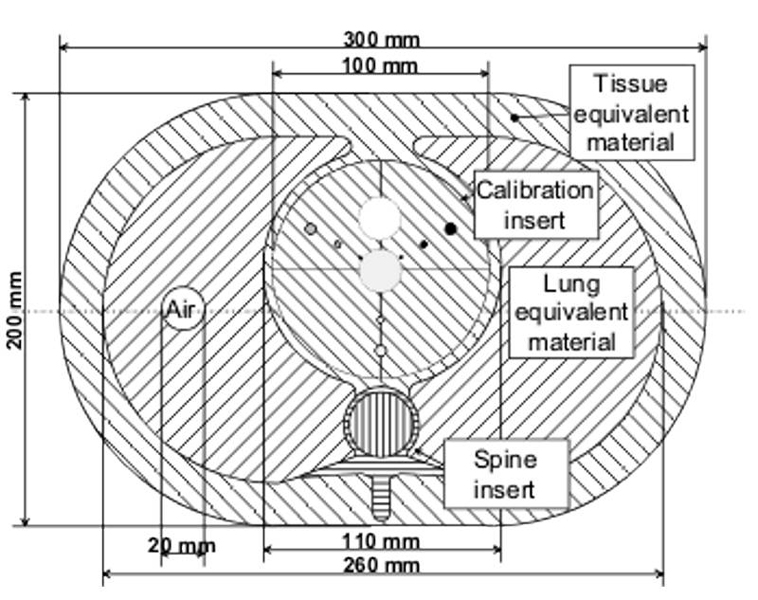
\includegraphics[width=0.95\linewidth]{./images/cardio_2.jpg}
  \captionof{figure}{QRM thorax phantom.}
  \label{fig:QRM_thorax}
\end{minipage}%
\begin{minipage}{.5\textwidth}
  \centering
  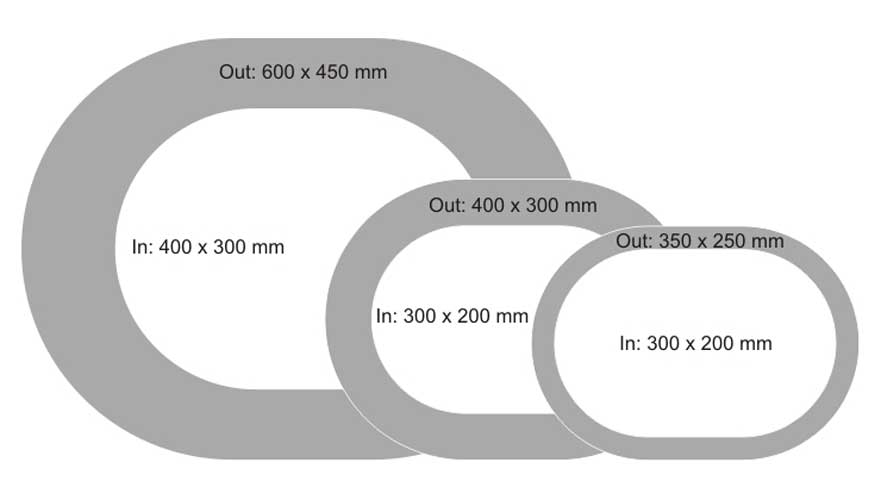
\includegraphics[width=0.95\linewidth]{./images/extension_2.jpg}
  \captionof{figure}{QRM thorax phantom extension rings.}
  \label{fig:QRM_extension}
\end{minipage}
\end{figure}

\section{External requirements}
\rrot{Determine how much noise output it may have.}
\rrod{Determine the height of the chair of the D-SPECT}
This section specifies the requirements that result from external influences.
\begin{table} [H]
\caption{External requirements (Textual)}
\label{tab:extreq_text}
\begin{tabular}{l|p{120mm}|}
	\makecell[l]{\textbf{Requirement} \\ \textbf{number}} & \multicolumn{1}{c}{\textbf{Description}}\\
	\hline
	TR-ERT01 & No high-density or "High-Z" material is to be used.\\ 
	TR-ERT02 & The phantom's left and front side must remain free, see figure \ref{fig:spect_surround}. \\ 
	\sout{TR-ERT03**} & \sout{Any part of the flow set-up and/or phantom, that does not fit directly on the patient chair, must remain horizontal with the remaining parts between 63 and 93cm.} \\
	\cline{2-2}
\end{tabular}
\raggedright

\end{table}

\begin{figure} [H]
  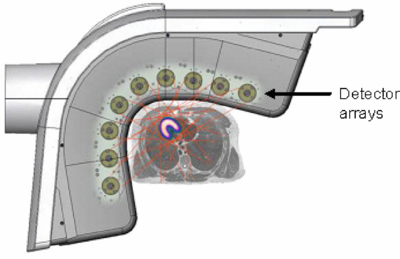
\includegraphics[width=0.5\linewidth]{./images/surrounding_spect.jpg}
  \caption{figure}{Schematic drawing of D-SPECT head\citep{erlandsson2009performance}.}
  \label{fig:spect_surround}
\end{figure}

\textbf{TR-ERT01} is based on material properties; "High-Z", or High-Density, material tend to block gamma radiation emitted by \ac{SPECT} tracers. Some examples of High-Z materials are Titanium (Ti), Chromium (Cr), Vanadium (V), Iron (Fe), or Lead (Pb).

\textbf{TR-ERT02} is based on the D-SPECTS design. The curved design allows for better patient comfort and proper imaging, but will require the phantom for being accessible, i.e. not blocked by High-Z materials, from the patient's left and front side.

\begin{table}[H]
\caption{External requirements (Quantitative)}
\label{tab:extreq_quan}
\begin{tabular}{l|p{65mm}ccp{20mm}|}
	\makecell[l]{\textbf{Requirement} \\  \textbf{number}} & \multicolumn{1}{c}{\textbf{Description}} & \multicolumn{1}{c}{ } & \multicolumn{1}{c}{\textbf{Value}} & \multicolumn{1}{c}{\textbf{Unit}} \\
	\hline	
	TR-ERQ01* &  Electric power. &  &  &  \\
	\hspace{1.5cm} A) & Supply voltage. 	& = 	& 230 	& Volt \\
	\hspace{1.5cm} B) & Supply current at TR-ERQ01 A). 	& < < 	& 6		& Ampere \\
	\hspace{1.5cm} C) & Supply type. 		& = 	& AC 	& - \\
	\hspace{1.5cm} C2) & Supply frequency	& =		& 50	& Hertz \\
	\cline{2-5}
\end{tabular} \\
\raggedright
\textit{* electric power connection (wall socket) for all systems, standard Dutch power mains. \textbf{No more than TR-ERQ01 B) can be drawn due to hospital safety measures.}}
\end{table}

\section{External interfaces}
This section specifies the requirements for the external interface, between user and set-up.
\begin{table} [H]
\caption{External interface requirements (textual)}
\label{tab:extint_text}
\begin{tabular}{l|p{120mm}|}
	\makecell[l]{\textbf{Requirement} \\ \textbf{number}} & \multicolumn{1}{c}{\textbf{Description}}\\
	\hline
	TR-EIT01 & Adjust output of flow generators. \\
	TR-EIT02 & Serial communication between control/monitoring systems and external interface.\\
	\cline{2-2}
\end{tabular}
\end{table}

\textbf{TR-EIT01} is based on the different experiments that need to be performed at different flow rates to determine the effect on the outcome.

\textbf{TR-EIT02} is based on the current control and monitoring system, which is connected via USB to the external interface running on in MATLAB on a laptop.

\begin{table}[H]
\caption{External interface requirements (Quantitative)}
\label{tab:extint_quan}
\begin{tabular}{l|p{65mm}ccp{20mm}|}
	\makecell[l]{\textbf{Requirement} \\  \textbf{number}} & \multicolumn{1}{c}{\textbf{Description}} & \multicolumn{1}{c}{ } & \multicolumn{1}{c}{\textbf{Value}} & \multicolumn{1}{c}{\textbf{Unit}} \\
	\hline	
	TR-EIQ01 &  Live plotting frequency of system's flow and pressure. & = &  10 & Hertz \\
	\cline{2-5}
\end{tabular} \\
\end{table}

\section{System qualities}
\rrot{Specify pressure threshold.}
This section specifies additional requirements that define the system's quality.
\begin{table} [H]
\caption{System qualities}
\label{tab:sysqual}
\begin{tabular}{l|p{120mm}|}
	\makecell[l]{\textbf{Requirement} \\ \textbf{number}} & \multicolumn{1}{c}{\textbf{Description}}\\
	\hline
	TR-SQT01 & Emergency shut down of flow set-up when arterial pressure exceeds TFR-GFQ07. \\ 
	TR-SQT02 & Emergency shut down of flow set-up when flow cannot be controlled, i.e. erratic or absent. \\
	TR-SQT03 & No reversed flow out of the phantom is allowed. \\
	\cline{2-2}
\end{tabular}
\end{table}

\textbf{TR-SQT01} and \textbf{TR-SQT02} are based on safety and prevention of leakage. Excessive pressure indicates faulty situation which must be resolved before components fail. Erratic, and especially the absence of proper flow, indicates a leakage and must be resolved. Leakage after injecting the tracer must be prevented at all costs.

\textbf{TR-QRT03} is based on optimisation of the experiments. Once the phantom is filled, it must remain filled such that experiments can be performed quickly in succession. 

\section{Constraints and Assumptions}
This section specifies the design constrains that have been imposed and the assumptions that have been made.

\begin{table}[H]
\caption{}
\label{tab:constassump}
\begin{tabular}{l|p{120mm}|}
	\makecell[l]{\textbf{Reference} \\ \textbf{number}} & \multicolumn{1}{c}{\textbf{Description}}\\
	\hline
	TR-CAT01 & Beating artefacts will not be generated. \\
	TR-CAT02 & Breathing artefacts will not be generated. \\
	TR-CAT03 & Hefty patients are simulated using extension rings on the thorax phantom.  \\
	\cline{2-2}
\end{tabular}
\end{table}

\textbf{TR-CAT01} and \textbf{TR-CAT02} are set to prevent over-complicating the first myocardial perfusion phantom. Breathing artefacts may be generated by means of a breathing thorax phantom, which is being developed in Münster, Germany. However, it will make the first phantom too complex. There is potential for the breathing phantom in the second iteration.

Extension rings can be used for the static thorax phantom, see TR-PRT01. These extension rings can increase the amount of "tissue" between the heart phantom (placed in the center) and the scanner. This will simulate more hefty patients, as stated by \textbf{TR-CAT03}.


% Appendix starts here
% change file name for better descriptive names, but start with apx-
\appendix
\chapter{Appendix 1} \label{app:one}


% Bibliography starts here
\backmatter

% Generate bibliography
\fancyhead[LO]{Bibliography}
\bibliographystyle{include/files/RaM-bibtex}
\label{ch:bib} %label to refer to
\bibliography{bibliography} 

\end{document}

